\documentclass[12pt]{article}

\usepackage{theorem,amsmath,amssymb}
\usepackage{graphicx}


\addtolength{\topmargin}{-23mm}
\addtolength{\textheight}{60mm}
\addtolength{\oddsidemargin}{-20mm}
\addtolength{\textwidth}{40mm}

\def\eqref#1{(\ref{#1})}
\newcommand{\goth}{\mathfrak}
\newcommand{\arrow}{{\:\longrightarrow\:}}
\def\1{\sqrt{-1}\:}
\newcommand{\restrict}[1]{{\left|_{{\phantom{|}\!\!}_{#1}}\right.}}

\renewcommand{\bar}{\overline}
\renewcommand{\phi}{\varphi}
\renewcommand{\epsilon}{\varepsilon}
\renewcommand{\geq}{\geqslant}
\renewcommand{\leq}{\leqslant}

\def\rad{\operatorname{\sf rad}}
\def\tr{\operatorname{\sf tr}}
\def\rk{\operatorname{\sf rk}}
\def\Alt{\operatorname{\sf Alt}}
\def\Sym{\operatorname{\sf Sym}}
\def\Id{\operatorname{\sf Id}}
\def\Hom{\operatorname{Hom}}
\def\Map{\operatorname{Map}}
\def\Gal{\operatorname{Gal}}
\def\Aut{\operatorname{Aut}}
\newcommand{\End}{\operatorname{End}}
\newcommand{\Mat}{\operatorname{Mat}}

\newcommand{\coker}{\operatorname{Coker}}

\def\chpoly{\operatorname{\sf Chpoly}}
\def\minpoly{\operatorname{\sf Minpoly}}

\def\cchar{\operatorname{\sf char}}

\def\Z{{\mathbb Z}}
\def\R{{\mathbb R}}
\def\C{{\mathbb C}}
\def\Q{{\mathbb Q}}
\def\N{{\mathbb N}}
\def\F{{\mathbb F}}

\def\Re{\operatorname{Re}}
\def\Im{\operatorname{Im}}

\makeatletter
\theoremstyle{definition}

\newtheorem{zadacha}{������}[section]
\newtheorem{opredelenie}{�����������}[section]
\newtheorem*{ukazanie}{��������}%[section]
\newtheorem*{zamechanie}{���������}%[section]

%\renewcommand{\labelenumi}{\ralph{enumi}.}
\renewcommand{\labelenumi}{\alph{enumi}.}
\newcommand{\subs}[1]{{\bigskip\centerline{\bf\large #1}\bigskip}}
\newcommand{\sttr}{{\bf(*)}}
\newcommand{\shrk}{{\bf(!)}}
\newcommand{\doublesttr}{{\bf(**)}}

\newcommand{\listok}[2]{%
\setcounter{page}{1}
\renewcommand{\@oddhead}{\hfil #2 \hfil}
\renewcommand{\@evenhead}{\hfil #2 \hfil}
\section*{#2}
\refstepcounter{section}
\setcounter{section}{#1}
}

\@addtoreset{equation}{section}
\renewcommand{\theequation}{\thesection.\arabic{equation}}

\let\oldllim=\lim
\def\lim{\oldllim\limits}
\makeatother


\newcommand{\diam}{{\sf diam}}
\theoremstyle{upshapenonumber}
\newtheorem{thms}{Theorem}
\begin{document}

%%%%%%%%%%%%%%%%%%%%%%%%%%%%%%%%%%%%%%%%%%%%%%%%
%To pass each sheet, it ...

%%%%%%%%%%%%%%%%%%%%%%%%%%%%%%%%%%%%%%%%%%%%%%%%


\listok{8}{GEOMETRY 8: Pointwise and uniform convergence}

%%%%%%%%%%%%%%%%%%%%%%%%%%%%%%%%%%%%%%%%%%%%%%%%
During the work on this sheet, it is allowed to use
Tychonoff's Theorem in the following form.  
\begin{thms} 
Let
$X$ be a compact topological space, $I$ an arbitrary set,
$X^I$ the topological space (in the pointwise convergence
topology), of the mappings $I\rightarrow X$. Then $X^I$ is
compact. 
\end{thms}

\begin{zadacha} 
Consider the space of of functions from an
interval to an interval.  Show that the limit of a sequence
of continuous functions need not be continuous.
\end{zadacha}

\begin{opredelenie}
Let $X$, $Y$ be metric spaces, 
$\{f_\alpha\}$ a set of continuous functions $X\rightarrow Y$.
Then $\{f_\alpha\}$ is called {\em uniformly continuous} if for 
any  $\epsilon$ there exists $\delta$ such that  
the image of any $\delta$-ball
under any $f_\alpha$ is contained in an
$\epsilon$-ball $B_\alpha$. (Note that 
$B_\alpha$ can depend upon $\alpha$.)
\end{opredelenie}

\begin{zadacha}
Let $f:\; X \arrow Y$ be a mapping of metric spaces that maps
each Cauchy sequence to a Cauchy sequence. Show that $f$ is
continuous as a mapping of topological spaces.
Is it true that any continuous mapping maps each Cauchy sequence
to a Cauchy sequence?
\end{zadacha}

\begin{zadacha}[!]
Let $X$, $Y$ be metric spaces, $\{f_i\}$ a uniformly continuous 
sequence of continuous functions $X\rightarrow Y$.
Suppose that  $\{f_i\}$ converges to $f$ in the 
pointwise convergence topology. Show that $f$ is continuous.
\end{zadacha}

\begin{ukazanie}
Show that  $f$ is uniformly continuous, 
with the same $\epsilon$, $\delta$ as
$\{f_i\}$, and then use the preceding problem.
\end{ukazanie}

Pick compact metric spaces
$X$, $Y$, 
and let $\Map(X,Y)$ be the set of continuous mappings
$X\rightarrow Y$. 

\begin{zadacha} 
For any $f, g\in \Map(X,Y)$ define
$$d_{\sup}(f,g):= \sup_{x\in X} d(f(x), g(x)).$$
Show the correctness of the definition of
$d_{\sup}(f,g)$, and that it defines a metric on
$\Map(X,Y)$.
\end{zadacha}

\begin{opredelenie}
The latter metric is called $\sup$-metric on 
$\Map(X,Y)$.
\end{opredelenie}

\begin{zadacha}[!]
Let a uniformly continuous sequence of mappings
$\{f_i\}\subset \Map(X,Y)$ pointwise converge to  
$f$. Show that it converges to  $f$ in the topology induced by the 
$\sup$-metric, too.
\end{zadacha}

\begin{ukazanie}
Let $\sup_{x\in X} d(f(x), f_i(x))>C$
for any $i$. Find a converging subsequence of 
$\{x_i\}$'s satisfying $d(f(x_i), f_i(x_i))> C$.
Let $x=\lim_{i\rightarrow\infty} x_i$.
Due to uniform convergence,
$d(f_i(x_i), f_i(x))\rightarrow 0$.
Derive a contradiction from the triangle inequality
\[ 
d(f_i(x), f(x)) + d(f_i(x_i), f_i(x)) \geq d(f(x), f_i(x_i)).
\]
\end{ukazanie}

\begin{zadacha}[!] 
(Arzel\`{a}-Ascoli Theorem)
Let $\Psi\subset\Map(X,Y)$
be closed (w.r.t. the $\sup$-metric) and
uniformly continuous. Show that $\Psi$ is compact.
\end{zadacha}

\begin{ukazanie}
Use Tychonoff's Theorem and the preceding problem.
As we have already said, we assume here that $X$ and $Y$ are compact!
\end{ukazanie}

\begin{zadacha}[**]
Find an independent of Tychonoff's Theorem (and thus, of the axiom 
of choice) proof of Arzel\`{a}-Ascoli Theorem.
\end{zadacha}

\begin{zadacha}[*]
Let $K\subset X$ be compact and $V\subset Y$ open.
Denote by $U(K,V)\subset \Map(X,Y)$ the set of all mappings
sending $K$ in  $V$. Consider the topology on $\Map(X,Y)$,
defined by the subbase of all $U(K,V)$. Show that it coincides with the
topology induced by the $\sup$-metric.
\end{zadacha}

\begin{opredelenie}
The latter topology on $\Map(X,Y)$
is called {\bf
topology of uniform convergence}. 
\end{opredelenie}

\begin{zadacha}
Show that the pointwise convergence topology is weaker than 
the uniform convergence topology; in other words that the
identity map from $\Map(X,Y)$ endowed with the latter topology onto
$\Map(X,Y)$ endowed with the former topology is continuous.
\end{zadacha}

\begin{opredelenie}
Let $M$ be a metric space and $Z\subseteq M$. 
{\bf Diameter} of $Z$ is the number 
$\diam(Z):= \sup_{x,y\in Z} d(x,y)$.
\end{opredelenie}

\begin{zadacha}
Let  $f \in \Map(X,Y)$ be an arbitrary mapping, 
$\epsilon$ be a real number, and $\delta(f, \epsilon)$ be 
the supremum of $\diam(f(B))$
over all the $\epsilon$-balls $B$ in $X$.
Show that  $\lim_{\epsilon \arrow 0}\delta(f, \epsilon)=0$.
\end{zadacha}

\begin{ukazanie} 
Assume that for a convergent to $0$ sequence
$\epsilon_i$, a collection of points
$x_i\in X$ and a positive constant $C$ one has $\diam
f(B_{\epsilon_i}(x_i)))>C$. 
Consider a limit point $x$ of $\{x_i\}$. Then each
$\epsilon$-ball around $x$ contains
$B_{\epsilon_i}(x_i)$ (for sufficiently large $i$),
implying that the image of this $\epsilon$-ball has diameter greater
than  $C$. Thus, $f$ is not continuous. 
\end{ukazanie}

\begin{zadacha}[!]
Let 
$f \in \Map(X,Y)$ be continuous. Show that $f$ is uniformly continuous.
\end{zadacha}

\begin{ukazanie}
The claim is tautologically equivalent to 
$\lim_{\epsilon \arrow 0}\delta(f, \epsilon)=0$.
\end{ukazanie}

\begin{zadacha} 
Let $\Psi \subset\Map(X,Y)$.
Show that $\Psi$ is uniformly continuous
if and only if 
$$\lim_{\epsilon\arrow 0}\sup_{f\in\Psi}\delta(f, \epsilon)=0.$$
\end{zadacha}

\begin{zadacha}[*]
Let $d_{\sup}(f,g) <\gamma$. Show that
$\delta(f, \epsilon)< \delta(g, \epsilon)+\gamma$.
\end{zadacha}

\begin{zadacha}[*]
Let $\{f_i\}$ be a Cauchy sequence in $(\Map(X,Y),d_{\sup})$.
Show that it is uniformly continuous.
\end{zadacha}

\begin{ukazanie}
We shall show that
\[
\lim_{\epsilon\arrow 0}\sup_{i}\delta(f_i,\epsilon)=0.
\]
Using the preceding problem, check that for all
$f_i$ in an  $\gamma$-ball in
$(\Map(X,Y),d_{\sup})$ the numbers $\delta(f_i, \epsilon)$
differ by no more than $\gamma$. Derive from this that 
$\sup_{i}\delta(f_i,\epsilon) <\delta(f_N,\epsilon)+\gamma$
for a fixed $N$, and thus
\[
\sup_{i}\delta(f_i,\epsilon)< \gamma + \max_{i\leq N}\delta(f_i,\epsilon)
\]
The limit of the latter, as $\epsilon \arrow 0$, cannot be greater
than $\gamma$, as all $f_i$ are uniformly continuous.
\end{ukazanie}

\begin{zadacha}[*]
Show the completness of the metric space $(\Map(X,Y),d_{\sup})$.
\end{zadacha}

\begin{zadacha}[*]
Is the space $(\Map(X,Y),d_{\sup})$ locally compact?
\end{zadacha}

%%%%%%%%%%%%%%%%%%%%%%%%%%%%%%%%%%%%%%%%%%%%%%%%
\subs{Peano curve}
%%%%%%%%%%%%%%%%%%%%%%%%%%%%%%%%%%%%%%%%%%%%%%%%

Let $[a,b]\subset \R$. The mapping
$[a,b] \overset{f}{\arrow} \R^n$ is called {\bf linear},
if $f (\lambda a + (1-\lambda) b)= \lambda f (a) +(1-\lambda) f(b)$,
for any $0<\lambda<1$. It is called {\bf piecewise linear}
if $[a,b]$ is partitioned into 
subsegments $[a, a_1], [a_1, a_2], [a_2, a_3], \ldots$, and
$f$ is linear on each of $[a_\ell,a_{\ell+1}]$.
The image of $[a,b]$ under a piecewise linear map is, certainly, 
a polygonal curve.

Let $f$ be a piecewise linear map
$f:[0, 1]\rightarrow [0, 1]\times [0, 1]$ satisfying the following
property;
all the segments of $f([0, 1])$ are parallel either to 
the line $x=y$ or to the line $x=-y$.
\begin{center}
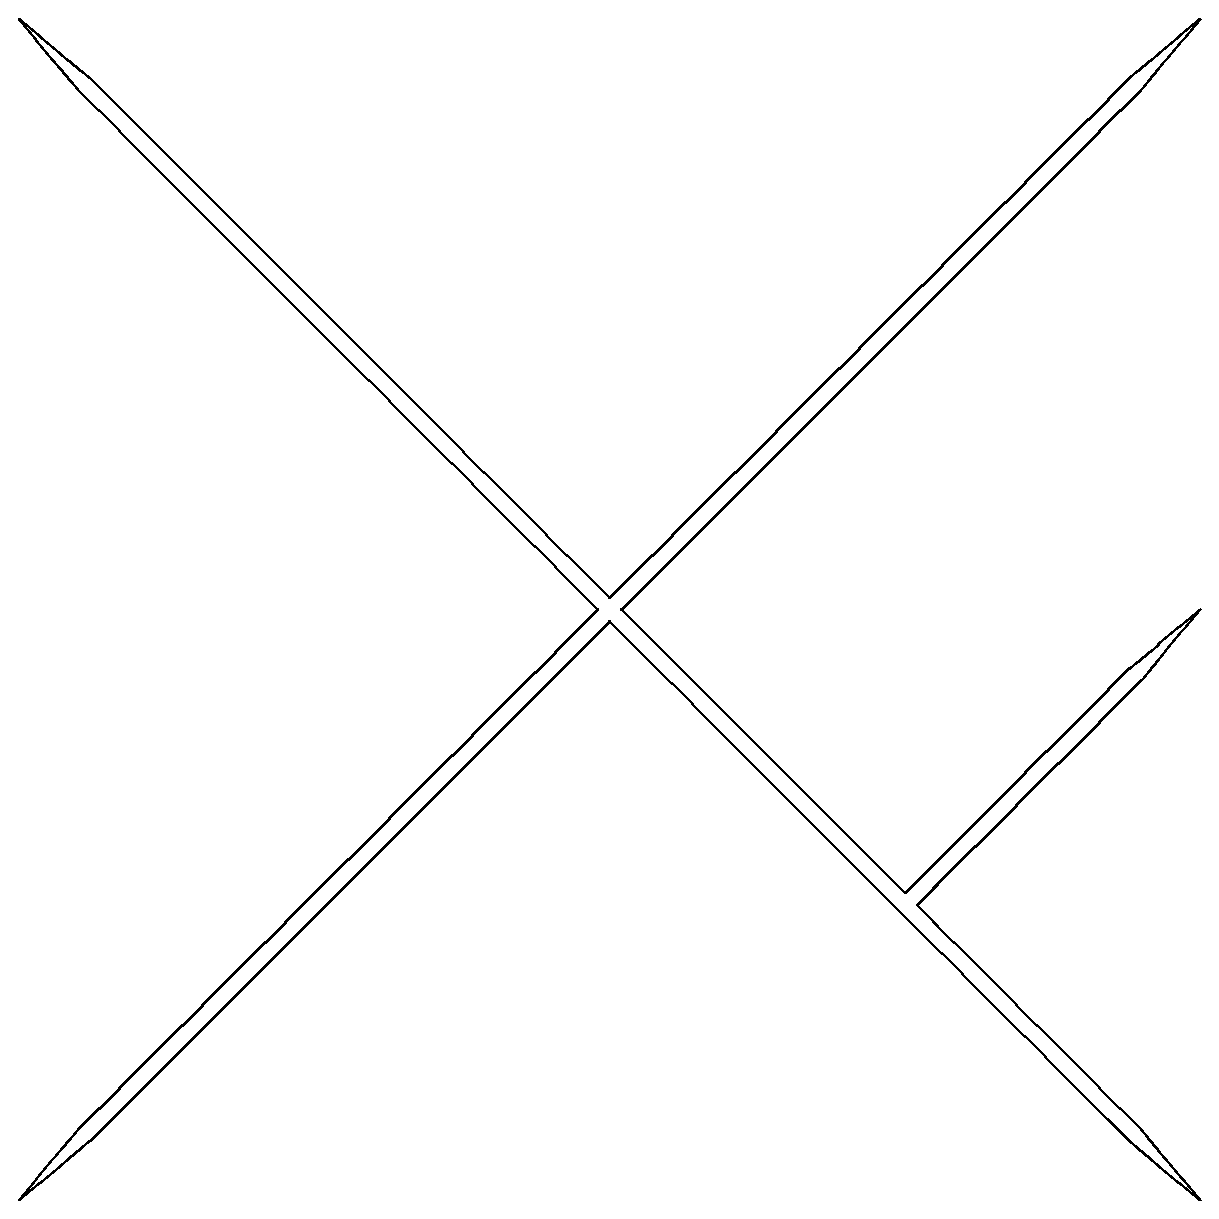
\includegraphics[height=60mm]{geom8pic0}
\end{center}
In other words, for any subsegment $[a, a_1]$, on which 
$f$ linear, $f$ maps
$[a, a_1]$ onto a diagonal of a square $Q$, with the sides parallel
to the coordinate axes. Let
${\cal P}l$ be the space of such piecewise linear mappings. 
Let us define an operation $\mu$ that produces from an
$f\in {\cal P}l$ with 
$k$ linear segments a piecewise linear map 
with $4k$ linear segments. 
%$$
%\begin{CD}
%\mbox{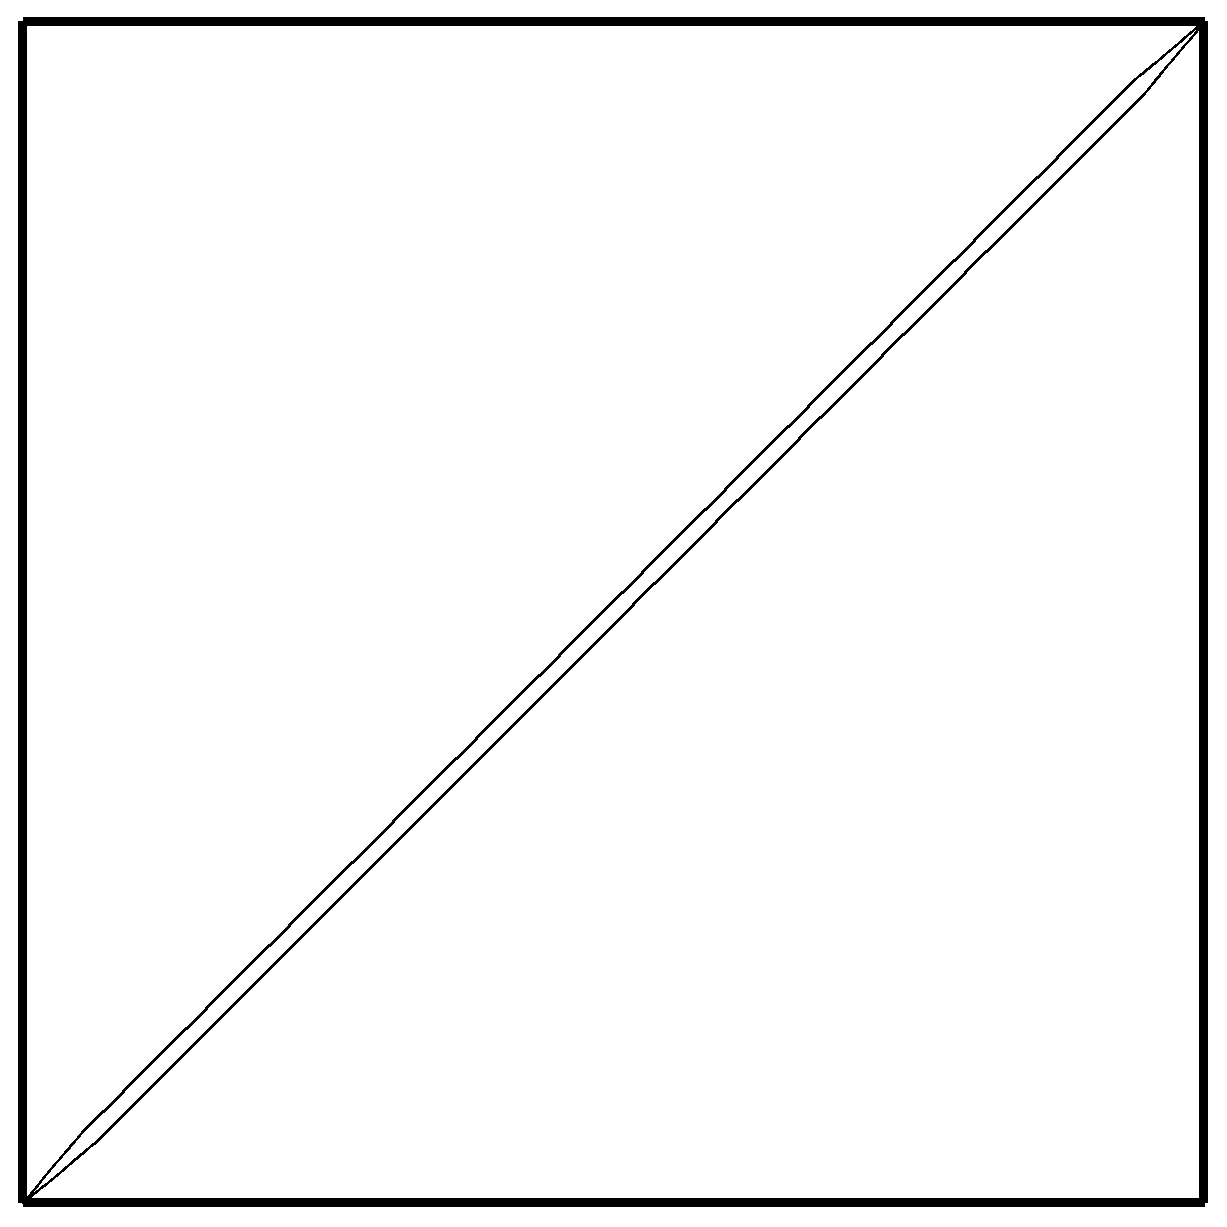
\epsfig{file=geom8pic1.eps,width=0.25\linewidth}}
%@>\mu>>
%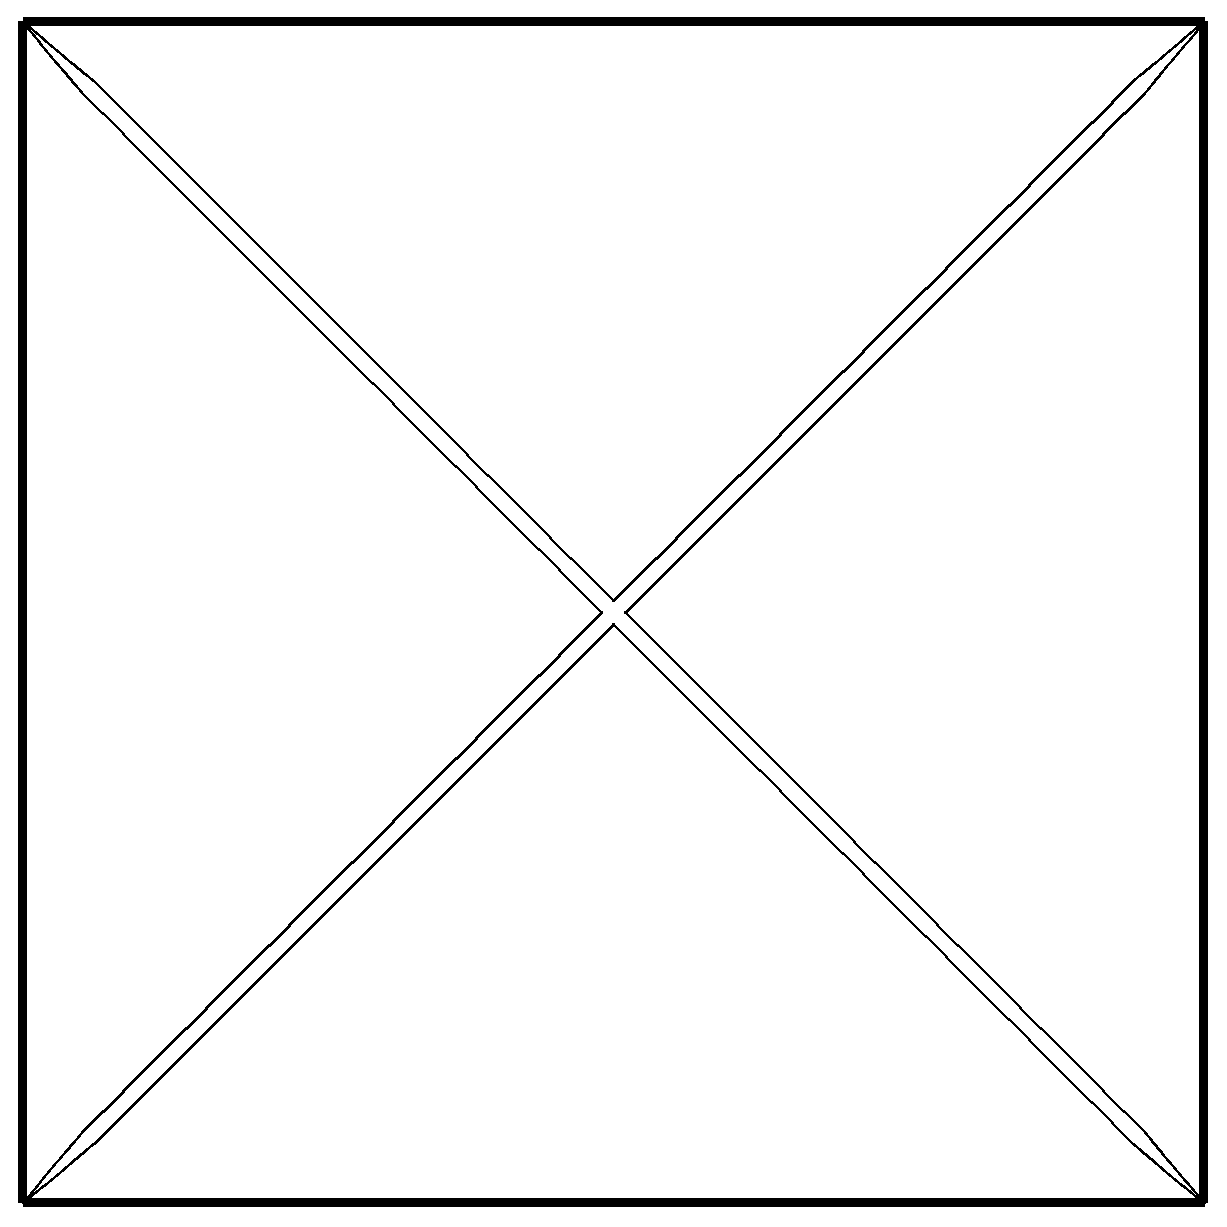
\epsfig{file=geom8pic2.eps,width=0.25\linewidth}
%@>\mu>>
%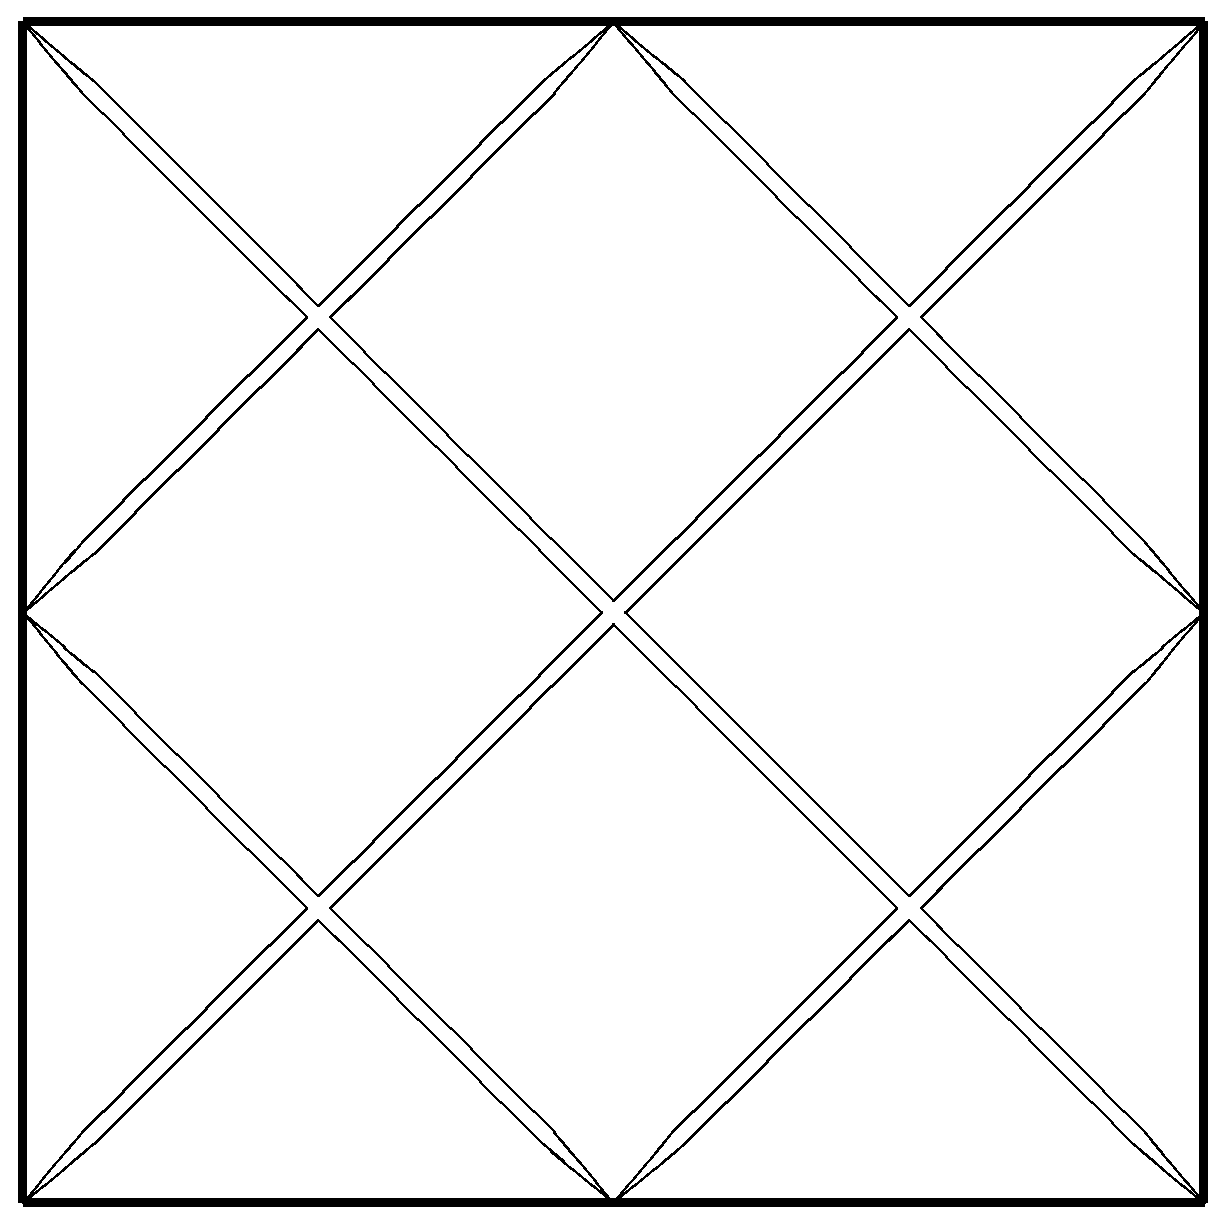
\epsfig{file=geom8pic3.eps,width=0.25\linewidth}
%\end{CD}
%$$
\begin{center}
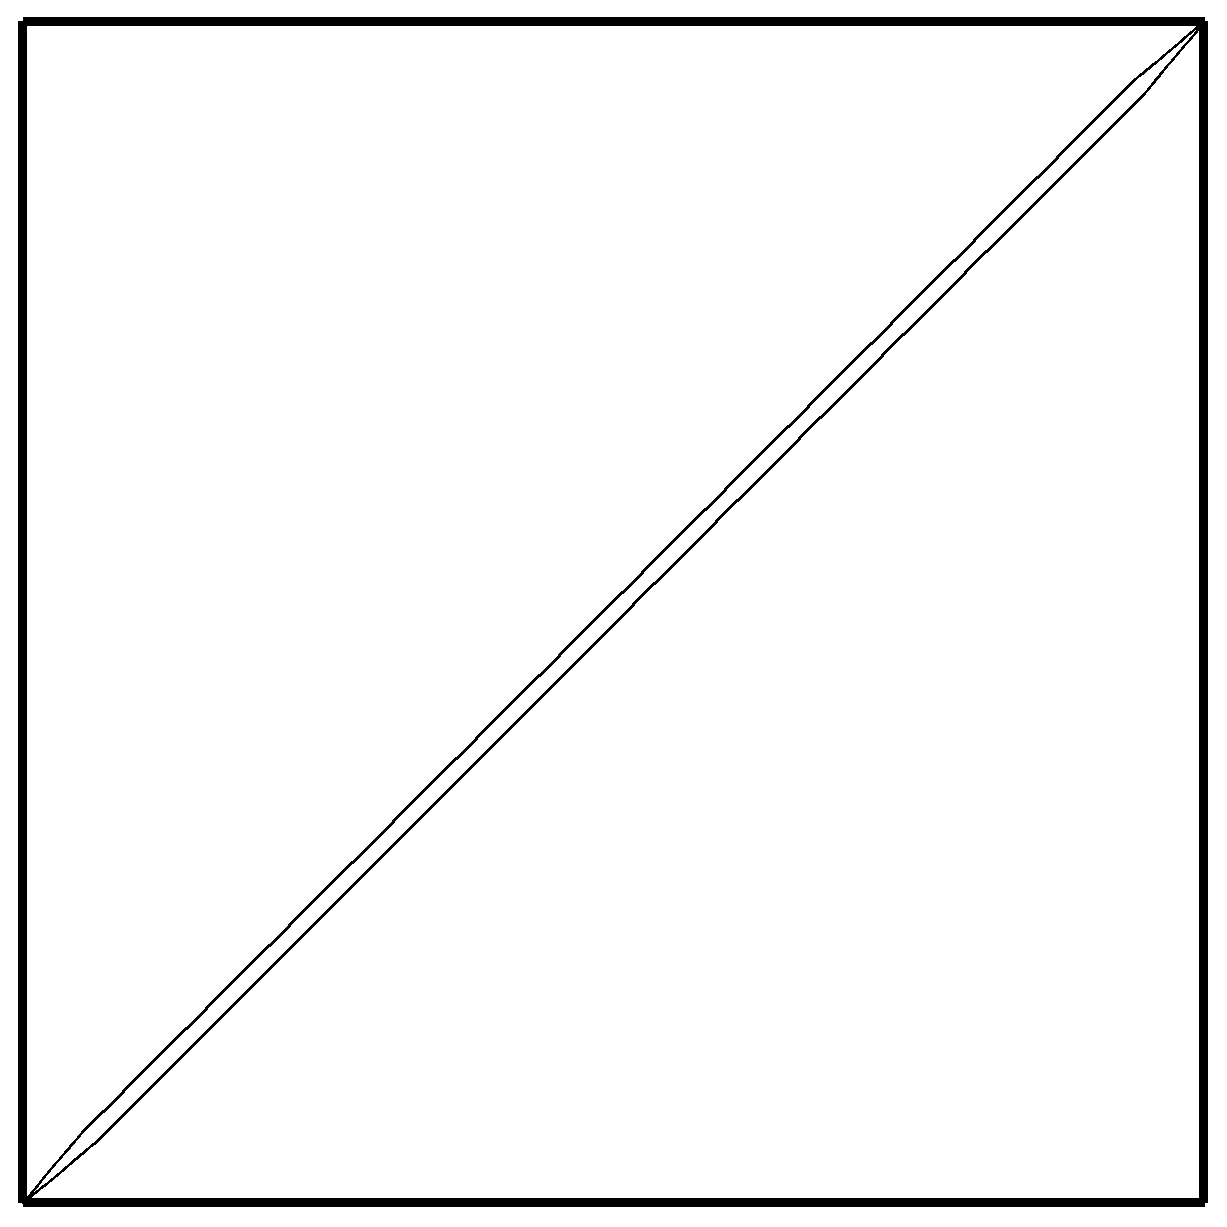
\includegraphics[height=40mm]{geom8pic1}%
$\overset{\mu}{\longrightarrow}$
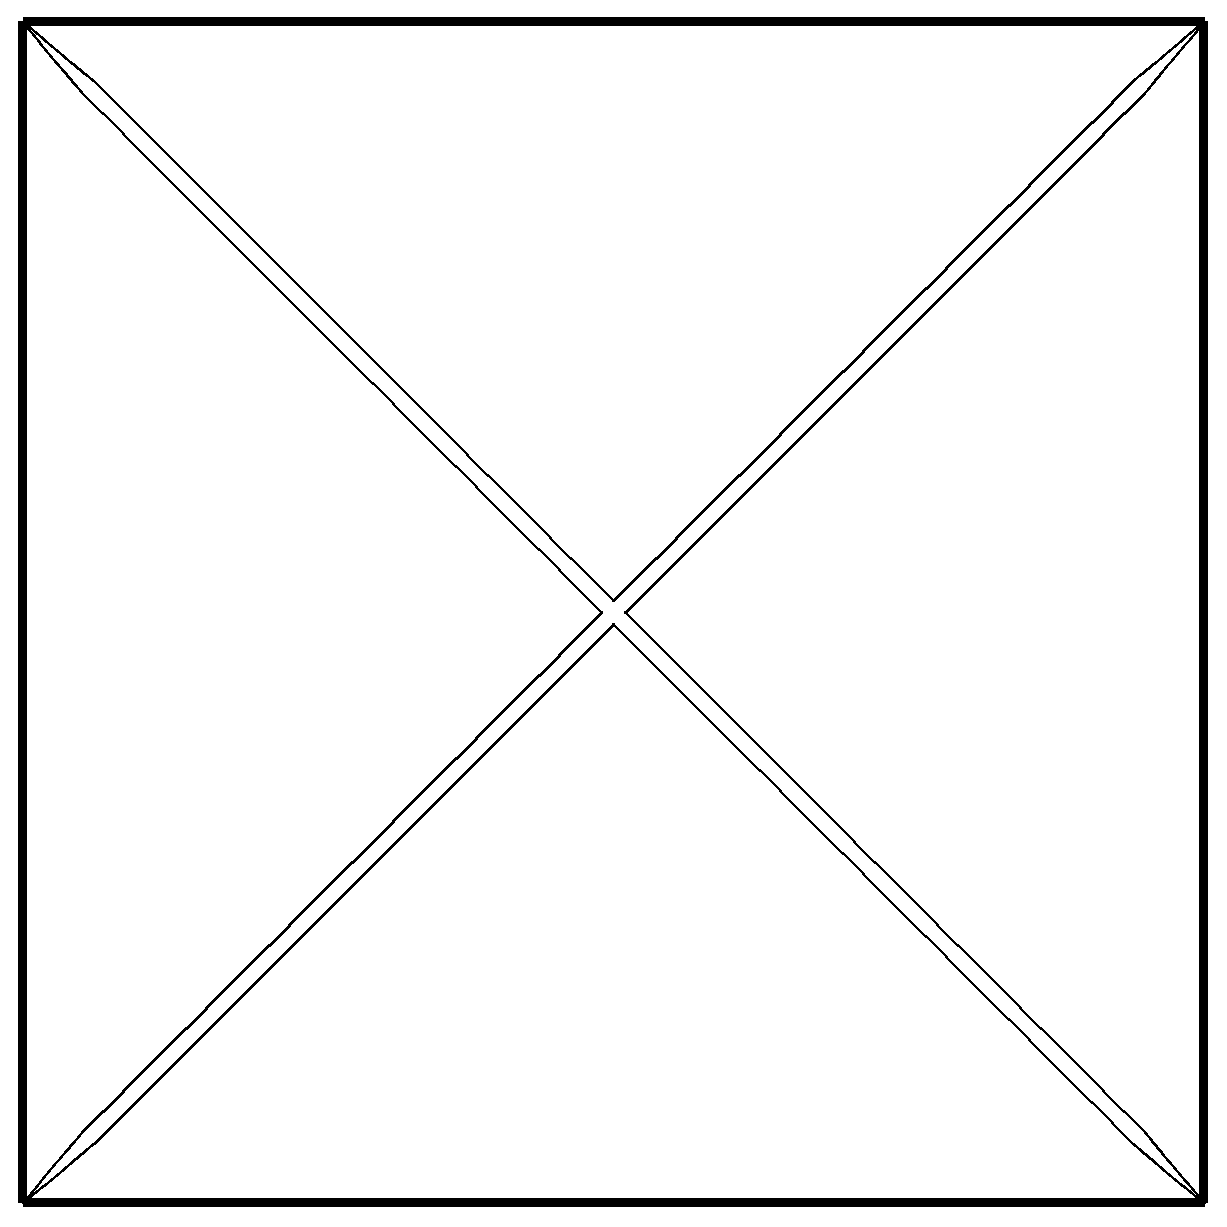
\includegraphics[height=40mm]{geom8pic2}%
$\overset{\mu}{\longrightarrow}$
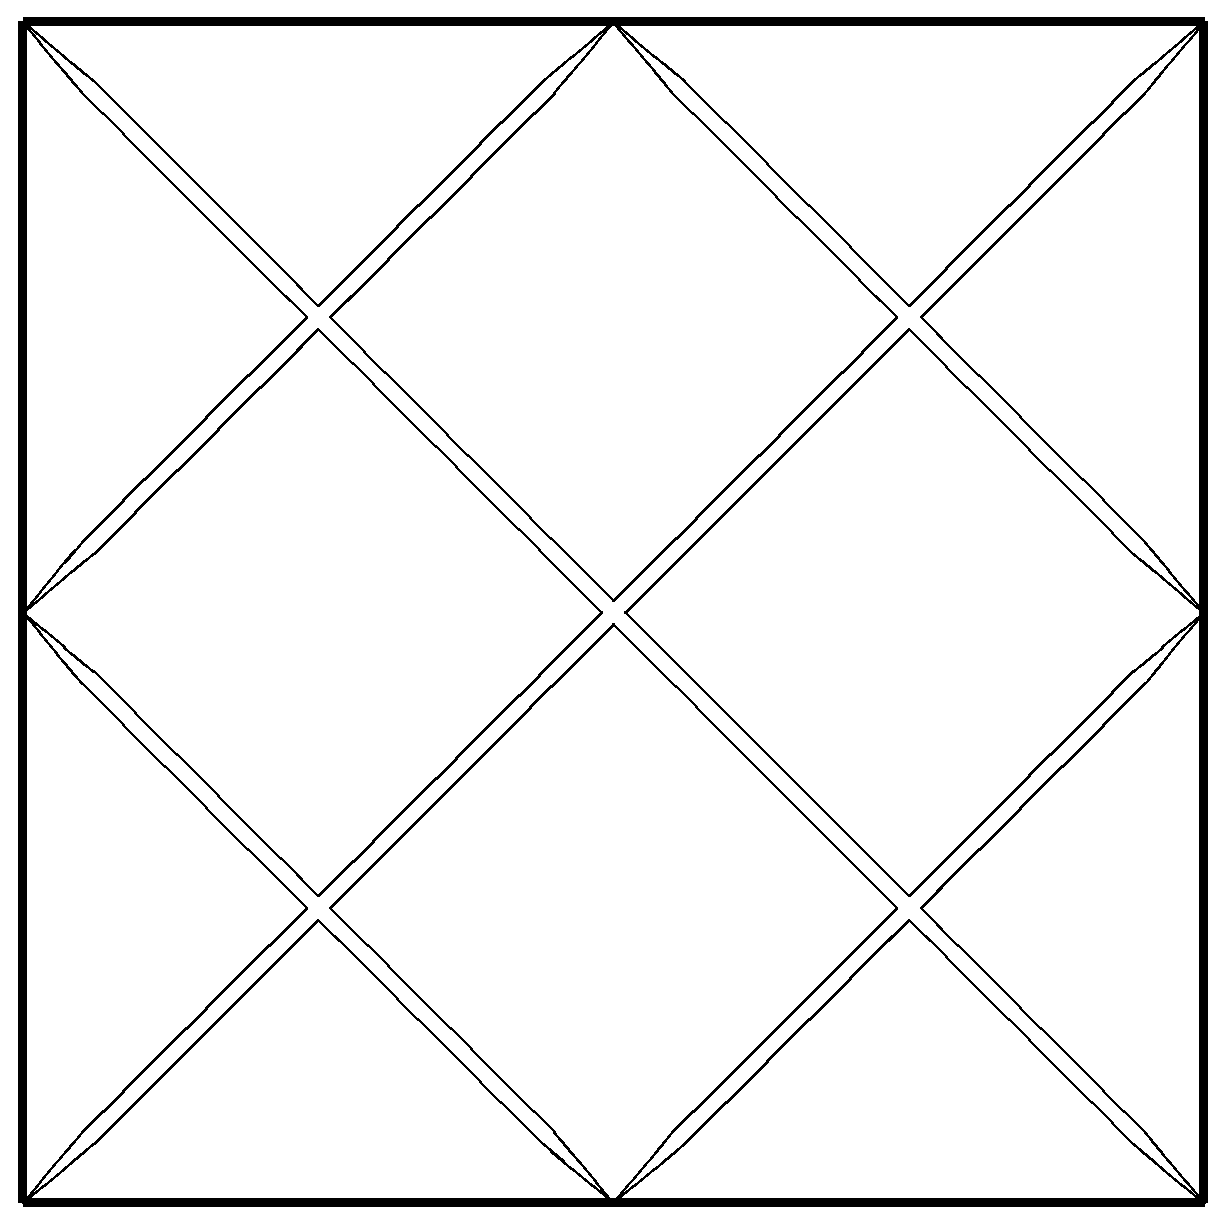
\includegraphics[height=40mm]{geom8pic3}%
\end{center}
Namely $\mu(f)$ is defined as follows.
\begin{enumerate}
\renewcommand{\labelenumi}{\arabic{enumi}.}
\item Denote by $a_0, a_1, \dots, a_k$ 
the ends of the segments where
$f$ was linear.
Then $\mu(f)$ maps $a_i$ to $f(a_i)$.

\item Partition each segment 
$[a_i, a_{i+1}]$ into 4 equal parts:
\[ 
  [b_{4i},b_{4i+1}], [b_{4i+1},b_{4i+2}], 
  [b_{4i+2},b_{4i+3}], [b_{4i+3},b_{4i+4}].
\]
$\mu(f)$ maps $[b_{4i},b_{4i+1}]$
linearly to $[f(a_i), f\left(\frac{a_i+a_{i+1}}2\right)]$,
and $[b_{4i+3},b_{4i+4}]$ to $[f\left(\frac{a_i+a_{i+1}}2\right), f(a_{i+1})]$.

\item Consider the square with a diagonal
$[f(a_i), f(a_{i+1})]$, and number its vertices clockwise:
$f(a_i)$, $A$, $f(a_{i+1})$, $B$. Then
$\mu(f)$ maps $[b_{4i+1},b_{4i+2}]$
linearly to $[f\left(\frac{a_i+a_{i+1}}2\right), B]$,
and $[b_{4i+2},b_{4i+3}]$ to $[B, f\left(\frac{a_i+a_{i+1}}2\right)]$.
\end{enumerate}
We obtain the following polygonal curve:
\begin{center}
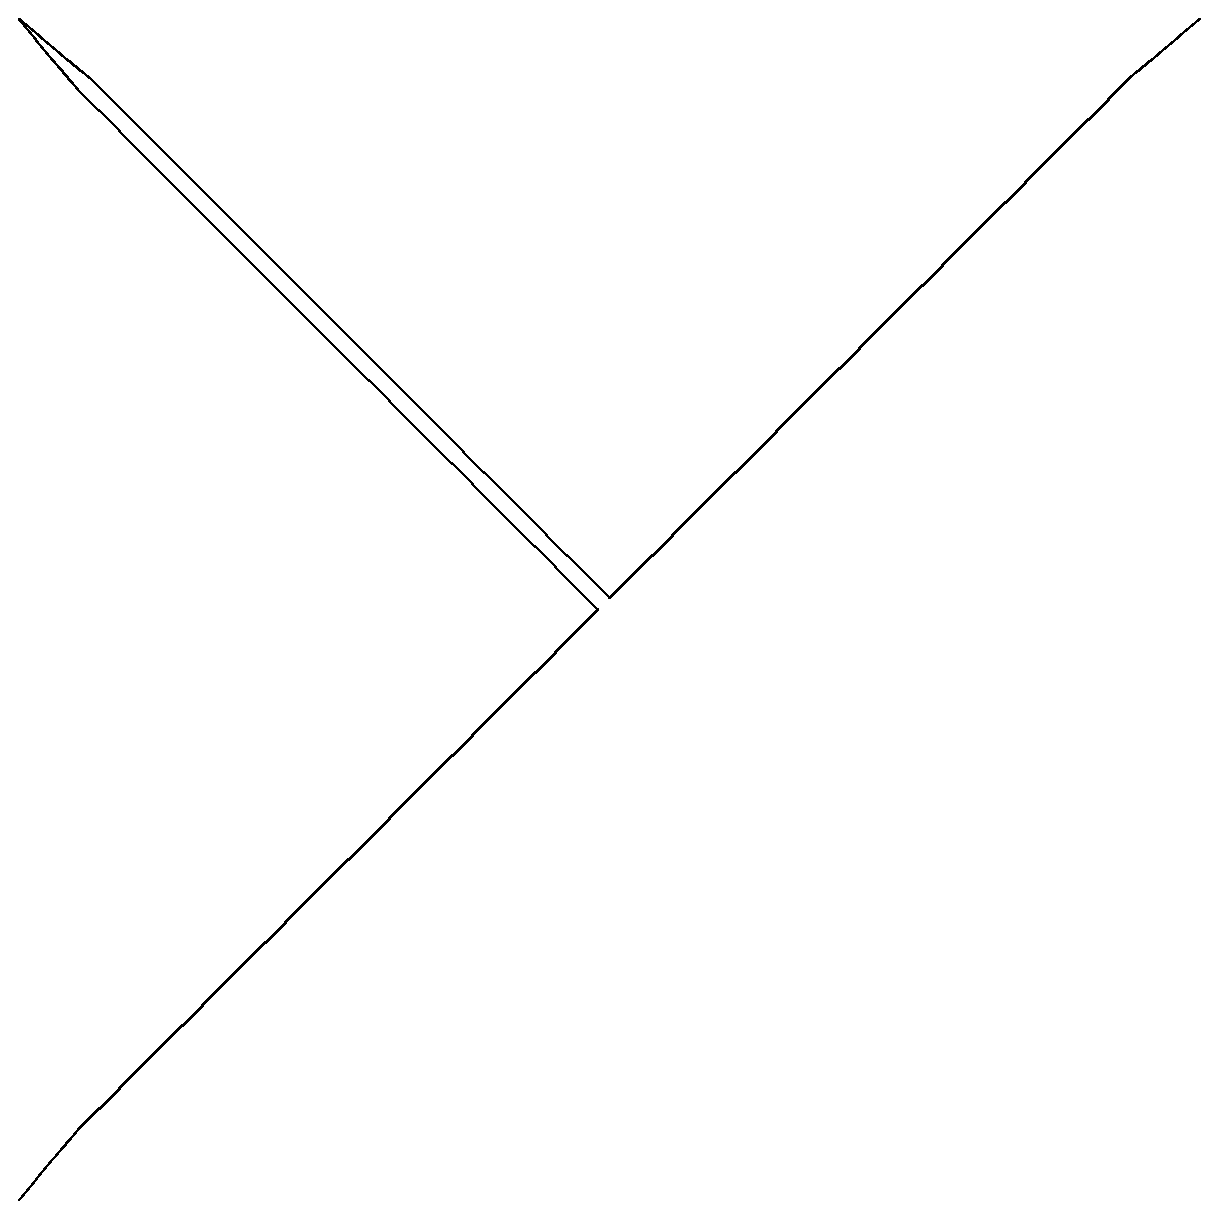
\includegraphics[height=60mm]{geom8pic4}%
\end{center}

\begin{zadacha}
Consider the segment and the square as metric spaces endowed with the standard
metric.
Let $f\in {\cal P}l$, and the biggest straight segment
$[f(a_i), f(a_{i+1})]$ of the corresponding polygonal curve
is of length $k$. Then $d_{\sup}(f, \mu(f)) \leq\frac{k}{\sqrt 2}$.
\end{zadacha}

\begin{zadacha} 
Let $f\in {\cal P}l$,  and the biggest straight segment
$[f(a_i), f(a_{i+1})]$ of the corresponding polygonal curve
is of length $k$. Then the biggest straight segment
in $\mu(f)$ is of length $k/2$.
\end{zadacha}

\begin{zadacha}
Let $f_0\in {\cal P}l$, $f_1 = \mu(f_0), \dots, f_n = \mu(f_{n-1})$,
and the biggest straight segment of the polygonal curve $f([0,1])$
has length $k$. Show that
\[
d_{\sup}(f_n, f_{n+1}) < \frac k {2^n \sqrt 2}
\]
\end{zadacha}

\begin{zadacha}[!]
Show that $\{ f_i\}$ is a Cauchy sequence in the metric 
$d_{\sup}$.
\end{zadacha}

\begin{zadacha} 
Let $f\in {\cal P}l$, and for all straight segments 
$[a_i, a_{i+1}]$ � $f$ the length of $[f(a_i), f(a_{i+1})]$
is at most \[ \rho(a_{i+1}-a_i),\] where $\rho>0$
is a real. 
Show that $\delta(f, \epsilon)\leq \rho\epsilon$,
where $\delta(f, \epsilon)$ is the function defined above. 
\end{zadacha}

\begin{zadacha}
Let $f_0\in {\cal P}l$, $f_1 = \mu(f_0), \dots, f_n = \mu(f_{n-1})$,
and for all straight segments
$[a_i, a_{i+1}]$ � $f_0$ the length of $[f(a_i), f(a_{i+1})]$
is at most $\rho(a_{i+1}-a_i)$.
Show that $\delta(f_n, \epsilon)\leq \rho 2^n\epsilon$.
\end{zadacha}

\begin{zadacha}
Let $f\in {\cal P}l$, and the longest straight segment
$[f(a_i), f(a_{i+1})]$ of $f([0,1])$ has length
$k$. Show that
$\delta(\mu(f), \epsilon) \leq 2\frac{k}{\sqrt 2}+\delta(f, \epsilon)$.
\end{zadacha}

\begin{zadacha} 
Let $f_0\in {\cal P}l$, $f_1 = \mu(f_0), \dots, f_n = \mu(f_{n-1})$,
and the longest straight segment of
$f_0([0,1])$ has length $k$.
Show that
\begin{equation}\label{_delta_Equation_}
\delta(f_n, \epsilon) \leq 4\frac{k}{2^{n-m}\sqrt 2}+\rho 2^m\epsilon
\end{equation}
for any $n$, $m$ ($n>m$)
\end{zadacha}

\begin{zadacha}
In the previous problem take $\epsilon < 2^{-2m}$,
$n > 2m$. Derive from  \eqref{_delta_Equation_} that
\[
\delta(f_n, \epsilon) \leq  \frac{4k\sqrt 2+\rho}{2^{-m}}.
\]
Show that for any $i$ the following holds.
\[
\delta(f_i, \epsilon) \leq  \max \left(\frac{4k\sqrt
2+\rho}{2^{-m}},  \rho 2^{2m}\epsilon\right).
\]
\end{zadacha}

\begin{zadacha}[!]
Let $f_0$ linearly map  $[0, 1/2]$ to the segment 
$[(0,0), (1,1)]$, and $[1/2, 1]$ -- to $[ (1,1), (0,0)]$.
Show that $\{ f_i\}$ is uniformly continuous.
\end{zadacha}

\begin{ukazanie}
Derive from the preceding problem that
$\lim_{\epsilon\arrow 0}\sup_i(\delta(f_i, \epsilon))=0$.
\end{ukazanie}

\begin{zadacha} 
Derive from Arzel\`{a}-Ascoli Theorem the existence of
$\lim f_i$ (in $\sup$-metric) and continuity of it as a 
function
${\cal P}:\; [0,1] \arrow [0,1]\times [0,1]$.
\end{zadacha}

\begin{opredelenie}
The function 
${\cal P}$ defined above is called a {\bf Peano curve}.
\end{opredelenie}

\begin{zadacha} 
Find ${\cal P}(q)$, for $q=\frac {a}{2^n}$ ($a\in \Z$).
(Such numbers are called binary-rational.)
\end{zadacha}

\begin{zadacha}
Let $Q_2$ be the set of binary-rational numbers.
Show that
${\cal P}(Q_2)$ is dense on the unit square. 
\end{zadacha}

\begin{zadacha}[!]
Show that ${\cal P}([0,1])$ is the whole unit square.
\end{zadacha}

\begin{ukazanie}
Use the fact that the image of a compact is compact.
\end{ukazanie}

\begin{zadacha}[!]
Is it possible to map, surjectively and continuously, 
$[0,1]$ onto a cube ? Onto a cube with one point removed?
\end{zadacha}

\end{document}
